\documentclass[11pt,a4paper]{article}
\usepackage[english]{babel}
\usepackage{fontspec}
\setmainfont{DejaVu Serif}
\setsansfont{DejaVu Sans}
\usepackage{geometry}
\geometry{left=25mm,right=23mm,top=22mm,bottom=22mm}
\usepackage{amsmath,amssymb,amsthm,booktabs,array,microtype,xcolor,hyperref,enumitem,fancyhdr}
\usepackage{graphicx}
\definecolor{navy}{HTML}{18354D}
\hypersetup{colorlinks=true,linkcolor=navy,urlcolor=navy,citecolor=navy}
\graphicspath{{figures/}}
\setlength{\parindent}{0pt}\setlength{\parskip}{3pt}
\pagestyle{fancy}\fancyhf{}
\fancyhead[L]{\small\sffamily CEX/DEX: seguimiento y liquidez}
\fancyhead[R]{\small\sffamily Revisión de dirección -- 29 oct. 2026}
\fancyfoot[C]{\thepage}
\title{\vspace{-1cm}\textbf{Seguimiento de precios y fragilidad de liquidez en mercados cripto híbridos CEX/DEX}\\[4pt]\large Un marco experimental basado en agentes y un modelo dinámico reducido\\[3pt]\normalsize Borrador preliminar para revisión de dirección}
\author{Edward Calderón\\\small Universidad Nacional de Colombia, Facultad de Minas\\\small Maestría en Ingeniería de Sistemas e Informática}
\date{29 de octubre de 2026}
\begin{document}
\maketitle
\section{Resumen}
Los mercados cripto híbridos combinan mecanismos centralizados de negociación con creadores automáticos de mercado descentralizados (AMM). El arbitraje puede reducir discrepancias entre precios, mientras que restricciones de ejecución, decisiones heterogéneas de negociación y cambios endógenos de liquidez pueden modificar la dinámica de ajuste. Se propone un marco metodológico con dos niveles: (i) un mapa discreto reducido cuyas variables son observables en el simulador; y (ii) un micromundo estocástico con un precio CEX de referencia, un AMM de producto constante y cuatro tipos de agentes. Simulaciones sintéticas preliminares verifican las direcciones mecánicas esperadas: el arbitraje acota el error de seguimiento, menor capacidad prolonga la recuperación y el retiro adaptativo de liquidez amplifica el impacto de una venta fija. Esas pruebas no validan el modelo frente a mercados reales ni convierten los coeficientes reducidos en parámetros empíricos. La investigación contrastará el mapa reducido con el ABM mediante escenarios controlados, sensibilidad y resultados de desacuerdo.
\textbf{Palabras clave:} seguimiento CEX/DEX; AMM; arbitraje; liquidez adaptativa; simulación multiagente; mapa discreto; reproducibilidad.
\section{Introducción}
Los intercambios descentralizados basados en creadores automáticos de mercado (AMM) y los mercados centralizados (CEX) representan mecanismos complementarios de formación de precios. Su interacción mediante arbitraje y diferencias de liquidez permite estudiar el seguimiento de precios y la respuesta a shocks. El aporte esperado no es una teoría general de estabilidad de mercados, sino un conjunto de mecanismos verificables en un simulador: qué parte de la corrección procede del arbitraje, cómo cambia con capacidad limitada y cómo la profundidad de liquidez transforma una venta de tamaño fijo. El modelo reducido se subordina a esa evidencia computacional y no se presenta como equivalente automático a un mercado real.

\section{Problema, pregunta e hipótesis}
\subsection{Problema científico}
No está suficientemente determinado, para el modelo mínimo propuesto, bajo qué combinaciones de capacidad de arbitraje, profundidad de liquidez, fricciones de ejecución y comportamiento de los agentes se logra seguimiento de precios, persiste una discrepancia o se amplifica una perturbación. Una simulación que solo grafique estos efectos no constituye por sí sola una explicación de las condiciones que los producen.
\subsection{Pregunta principal}
\emph{¿Bajo qué condiciones de arbitraje, liquidez y comportamiento heterogéneo un mercado híbrido CEX/DEX simplificado reduce o mantiene un error de seguimiento acotado, y en qué medida un mapa discreto reducido describe los regímenes observados en un micromundo multiagente estocástico?}
\subsection{Hipótesis de trabajo}
El seguimiento depende del balance entre realimentación correctiva (arbitraje) y mecanismos potencialmente amplificadores (presión de negociación y liquidez adaptativa). La variación de estos mecanismos produce regiones de comportamiento distinguibles con métricas experimentales; el mapa reducido sirve como diagnóstico local y debe fallar explícitamente cuando sus hipótesis dejan de ser razonables.
\textbf{H1a.} Bajo supuestos definidos de capacidad, latencia y costes, el arbitraje reduce las discrepancias posteriores a una perturbación aislada.\\
\textbf{H1b.} La retirada proporcional de liquidez aumenta el impacto de una operación posterior de tamaño fijo; ciertas reglas adaptativas de LP amplifican shocks en comparación con un contrafactual de liquidez estática.\\
\textbf{H1c.} Un mapa discreto estimado o diagnosticado alrededor de una región de operación puede clasificar parcialmente la contracción o persistencia del error en el ABM; los desacuerdos son un resultado que delimita su validez.
\section{Objetivos}
\textbf{General.} Desarrollar y evaluar un marco computacional para analizar seguimiento CEX/DEX y fragilidad de liquidez, combinando un mapa dinámico reducido trazable con simulación basada en agentes heterogéneos.
\begin{enumerate}[leftmargin=*,itemsep=2pt]
\item Formalizar el estado, los mecanismos de transacción del AMM, el arbitraje y las políticas de los cuatro agentes con especificación ODD.
\item Construir un mapa discreto reducido con banda de no arbitraje y variables observables en el ABM; evaluar contracción local y condiciones de estabilidad de la linealización solo en las regiones donde aplique.
\item Implementar y verificar un simulador reproducible con reservas, inventarios, costes y eventos ordenados de forma explícita.
\item Diseñar experimentos factoriales o de sensibilidad para shocks, intensidad de arbitraje, profundidad y respuesta de LP.
\item Contrastar resultados teóricos y simulados, incluyendo regiones de desacuerdo, robustez estadística y límites de extrapolación.
\end{enumerate}
\section{Modelo de mercado y observables}
Sea $p_t^C>0$ el precio externo CEX y $p_t^D>0$ el precio marginal del AMM. En una piscina de producto constante sin comisiones durante el swap, $x_ty_t=k_t$ y $p_t^D=y_t/x_t$. Se define el error logarítmico de seguimiento
\begin{equation}
e_t=\log(p_t^D/p_t^C),\qquad D_t=(|e_t|-\gamma_t)_+,
\end{equation}
donde $\gamma_t\ge 0$ representa una banda de no arbitraje operativa, cuyos costes, orientación y dependencia del tamaño de operación deben justificarse. El conjunto $\mathcal{E}_{\gamma}=\{e:|e|\leq\gamma\}$ no es lo mismo que el equilibrio puntual $e=0$.
Para una venta de $q>0$ unidades del activo $x$ en un AMM ideal sin comisiones:
\begin{equation}
p^{D\prime}=\frac{p^D}{(1+q/x)^2},\quad \Delta\log p^D=-2\log(1+q/x).
\end{equation}
Si un LP retira proporcionalmente las reservas dejando $r x,r y$, $0<r<1$, el precio marginal inmediato no cambia; el impacto de la misma venta sí aumenta. Las reglas para entradas/salidas de LP y comisiones distinguen transacciones que mantienen $xy=k$ de aquellas que modifican $k$.
\subsection{Modelo completo}
\begin{equation}
S_{t+1}=F(S_t,\xi_t,J_t;\theta),
\end{equation}
con estado que incluya precios, reservas, inventarios, cuentas, memoria requerida por políticas, y variables de liquidez; $\xi_t$ son innovaciones aleatorias, $J_t$ shocks experimentales y $\theta$ parámetros. Las métricas principales son error excedente, recuperación sostenida, respuesta máxima, profundidad, slippage, frecuencia de cascadas y sensibilidad a semillas. El CEX permanece \emph{exógeno}; no se afirmará contagio bidireccional.
\section{Mapa reducido trazable y criterios locales}
\subsection{Por qué se reemplaza la ODE inicial}
El borrador anterior proponía una ODE con funciones hiperbólicas y argumentos Lyapunov/ISS antes de contar con una simulación que conectara sus estados y coeficientes con swaps, capacidad de arbitraje o reglas de LP. Esa formulación es prematura: el ABM se ejecuta por ticks y eventos discretos, y una ODE no obtiene validez por ser matemáticamente conveniente. En esta versión se reemplaza como núcleo del manuscrito por un mapa discreto cuya semántica coincide con el orden de actualización del simulador.

\subsection{Mapa discreto de seguimiento}
Se define el exceso con signo respecto de la banda de no arbitraje:
\begin{equation}
d_t=\operatorname{sgn}(e_t)(|e_t|-\gamma)_+.
\end{equation}
Sea $z_t$ la presión neta de compra en el DEX, positiva cuando eleva $p_t^D$, y $u_t=-\Delta\log p_t^C$ el desplazamiento inducido por la referencia CEX. Una aproximación local candidata, que deberá contrastarse con datos del ABM y no imponerse sobre ellos, es
\begin{align}
d_{t+1}&=(1-\alpha)d_t+\beta z_t+u_t+\varepsilon_t,\\
z_{t+1}&=-\chi d_t+\rho z_t+\eta_t.
\end{align}
Aquí $\alpha\ge0$ representa corrección efectiva de arbitraje, $\beta>0$ el impacto local de presión de compra, $\chi\ge0$ una realimentación correctiva hacia la banda y $\rho$ la persistencia de presión. Todos son parámetros de una aproximación local, no constantes universales de mercado.

Sin entradas ni ruido, la linealización es
\begin{equation}
\begin{pmatrix}d_{t+1}\\z_{t+1}\end{pmatrix}=
A\begin{pmatrix}d_t\\z_t\end{pmatrix},\qquad
A=\begin{pmatrix}1-\alpha&\beta\\-\chi&\rho\end{pmatrix}.
\end{equation}
Para este mapa $2\times2$, la estabilidad local de Schur requiere que las raíces de $A$ estén dentro del círculo unitario; equivalentemente,
\begin{equation}
1-\det(A)>0,\qquad 1-\operatorname{tr}(A)+\det(A)>0,\qquad 1+\operatorname{tr}(A)+\det(A)>0.
\end{equation}
Estas desigualdades son un criterio diagnóstico del mapa reducido. No prueban estabilidad del ABM con ruido, saturaciones, límites de capital, cambios de liquidez o agentes adicionales.
\subsection{Regímenes de operación y uso acotado de modelos múltiples}
Medina et al. \cite{medina2009} describen una dinámica no lineal mediante modelos lineales locales asociados a puntos de operación. Esta tesis no adopta su componente de diagnóstico de fallas ni intenta identificar un sistema financiero real. El antecedente se usa de manera acotada para documentar escenarios CEX con regiones operativas explícitas ---referencia normal, shock y recuperación---, cada una con parámetros declarados de perturbación y ejecución. La separación permite evaluar sensibilidad sin afirmar que los regímenes sean una estimación empírica ni añadir una nueva clase de agente.
\subsection{Mecánica exacta que ancla el mapa}
La forma discreta se vincula al AMM mediante una identidad verificable. Si el DEX recibe una venta de $q>0$ unidades de $x$, entonces $\Delta\log p^D=-2\log(1+q/x)$. Un arbitrajista que actúa cuando $|e|>\gamma$ intenta llevar el precio a la banda, pero su fracción de reserva negociable está limitada por capacidad. Por tanto, $\alpha$ no se postula como una ganancia abstracta: se estima o se diagnostica a partir de la contracción observada del exceso $d_t$ por tick. La liquidez entra de manera directa porque la misma venta absoluta aumenta $q/x$ cuando el LP retira reservas.
\section{Diseño experimental y falsación}
\begin{table}[ht]
\centering\small
\begin{tabular}{p{.08\linewidth}p{.33\linewidth}p{.46\linewidth}}
\toprule ID & Intervención controlada & Contrafactual y pregunta \\\midrule
E0 & Referencia constante, LP fijo, arbitraje activado/desactivado & Verificar existencia y naturaleza de un régimen de seguimiento.\\
E1 & Shock exógeno del precio CEX; variar capacidad, costes y retardo & Medir error, cota, tiempo de retorno sostenido y resiliencia.\\
E2 & LP estático contra LP adaptativo sensible a volatilidad & Distinguir impacto mecánico de menor profundidad de la realimentación endógena.\\
E3 & Presión de ventas/reacciones heterogéneas, mismo shock externo & Identificar amplificación, persistencia y límites de la aproximación analítica.\\
\bottomrule
\end{tabular}
\end{table}
El diseño utilizará pares de semillas comunes cuando sean compatibles, barridos reducidos, análisis de sensibilidad con intervalo de incertidumbre, y preregistro de criterios de clasificación. El número de réplicas se fijará mediante convergencia y precisión del estimador, no solo mediante una regla universal de treinta. Para evitar sesgo por exploración, las configuraciones de confirmación estarán separadas de las de selección.
\subsection{Simulaciones preliminares: comprobación de mecanismos}
Se implementó un prototipo sintético reproducible de CPMM, flujo de traders, arbitraje acotado y LP adaptativo. Se ejecutaron 100 semillas por variante. En E0--E2 se desactivó el ruido intencionalmente para probar comparativos mecánicos; por ello las repeticiones coinciden y no deben interpretarse como evidencia estadística independiente. E3 sí incluye ruido, tendencia y reacción de pánico. No se usaron datos de mercado: los resultados son una verificación interna de dirección, no validación externa.

\begin{table}[ht]
\centering\small
\caption{Resultados preliminares sintéticos (medianas de 100 ejecuciones por variante). Error: $|\log(p^D/p^C)|$.}
\begin{tabular}{p{.11\linewidth}p{.24\linewidth}p{.22\linewidth}p{.29\linewidth}}
\toprule Escenario & Contrafactual & Resultado observado & Lectura limitada \\ \midrule
E0 & Arbitraje activo / apagado & Error máximo $0.0409/0.1000$; retorno a banda en $2$/no observado ticks & La corrección acotada reduce el error tras un shock.\\
E1 & Capacidad alta / baja & Retorno a banda en $1/9$ ticks; error máximo $0.0030/0.1080$ & La capacidad de arbitraje importa en la velocidad de recuperación.\\
E2 & LP estático / adaptativo & Impacto de venta fija $0.0940/0.2032$; liquidez mínima $10000/4500$ & Menor profundidad aumenta el impacto de la misma venta absoluta.\\
E3 & Liquidez estática / adaptativa & Máximo error $0.0660/0.3719$; ticks de retorno $3/33$ & La regla LP adaptativa puede amplificar una cascada bajo estas condiciones.\\
\bottomrule
\end{tabular}
\end{table}

En una cuadrícula local de excesos iniciales y órdenes pequeñas, la proyección por mínimos cuadrados de $d_{t+1}\approx k d_t$ produjo $\hat{k}=0.1874$ bajo $\gamma=0.003$ y capacidad máxima de arbitraje del $3\%$ de la reserva por tick; esto equivale a una contracción diagnóstica $\hat{\alpha}=1-\hat{k}=0.8126$. No se reporta como parámetro calibrado: cambia con la banda, la capacidad, el tamaño de la orden y las no linealidades del AMM. Su utilidad en esta etapa es mostrar que la ecuación reducida puede ser medida contra el propio mecanismo y no solo propuesta de forma abstracta.

\begin{figure}[ht]
\centering
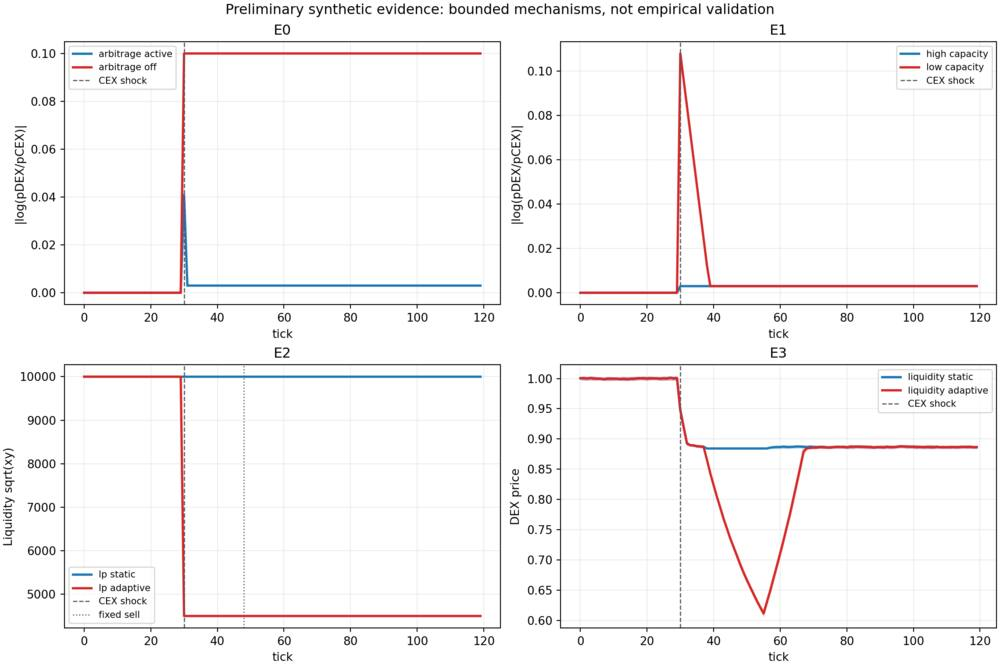
\includegraphics[width=\linewidth]{preliminary_evidence.jpg}
\caption{Evidencia sintética preliminar. E0 y E1 muestran el error de seguimiento; E2 muestra el retiro de liquidez antes de una venta fija; E3 muestra la amplificación transitoria bajo la regla LP adaptativa. Las bandas representan percentiles 25--75 donde existe variación por semilla.}
\label{fig:preliminary}
\end{figure}

Estos resultados respaldan mantener H1a y H1b como hipótesis operativas. H1c permanece abierta: aún falta diseñar una clasificación ex ante de los regímenes del ABM, estimar el mapa en una muestra de selección y evaluarlo en configuraciones de confirmación separadas.
\section{Playground reproducible y transferencia tecnológica}
\subsection{Arquitectura}
Un motor determinista de eventos ejecutará el AMM, arbitraje, políticas y contabilidad. El generador pseudoaleatorio se fijará y sus flujos se separarán por componente; los shocks y el orden de ejecución serán configurables y registrados. Cada corrida producirá `run-id', archivo de configuración, commit SHA, versión de entorno, semillas, series temporales, métricas, validación de invariantes y suma criptográfica de artefactos.

\subsection{Referencia canónica de implementación}
La referencia pública y versionada de la arquitectura es el repositorio \emph{Master-s-thesis} \cite{calderonrepo2026}, disponible en \href{https://github.com/edwardcalderon/Master-s-thesis}{\texttt{repositorio Master-s-thesis}}. En esta versión, el manuscrito compilable se publica en \href{https://github.com/edwardcalderon/Master-s-thesis/tree/main/thesis/preprint}{\texttt{thesis/preprint}}; el prototipo CPMM y su análisis se publican en \href{https://github.com/edwardcalderon/Master-s-thesis/tree/main/experiments/cex_dex_preliminary}{\texttt{experiments/cex\_dex\_preliminary}}. Los destinos de estos enlaces identifican la arquitectura y sus versiones; los artefactos de cada ejecución conservan además su propio \emph{commit SHA}, configuración y semilla. Ninguna rama, URL ni resultado sintético se interpreta como evidencia empírica de mercado.
\subsection{Contratos de reproducción}
\begin{enumerate}[leftmargin=*,itemsep=1pt]
\item Configuraciones YAML versionadas, unidades económicas especificadas y dependencias bloqueadas (`uv.lock' o equivalente).
\item Pruebas de swaps, reservas positivas, inventarios y conservación neta, con reglas explícitas para comisiones y retiros.
\item Comandos estables: `run one', `run sweep', `analyze', `verify' y `reproduce figure'. El prototipo actual se reproduce ejecutando \texttt{python3}, seguido de la ruta \url{experiments/cex_dex_preliminary/cex_dex_preliminary.py}, con los argumentos \texttt{--output} \url{output/preliminary_simulations} \texttt{--seeds 100}.
\item CI con simulaciones de referencia y tolerancias numéricas documentadas; resultados extensos en almacén de artefactos, no necesariamente en Git.
\item Dataset sintético como referencia primaria y conjunto empírico acotado con licencia, procedencia, timestamps y scripts de ingestión.
\end{enumerate}
\subsection{Relación con software de mercado abierto}
El mercado teórico básico seguirá la mecánica CPMM compatible con un AMM tipo Uniswap v2 \cite{uniswap2020,angeris2020}; no se extrapolará sin pruebas a posiciones concentradas de Uniswap v3/v4. Se propone verificar swaps contra contratos de referencia desplegados localmente con Foundry/Anvil y librerías Web3, bajo configuración controlada y sin dinero real. Para la referencia CEX se podrán utilizar series públicas obtenidas con adaptadores de mercado como CCXT o API pública del exchange, verificando licencias, identidad del par, latencia, spreads y timestamp. Un segundo nivel, opcional, consiste en replay de eventos on-chain indexados (p. ej. registros de swaps y Sync de pools compatibles) para validar la magnitud del error de ejecución. No se requiere correr nodos mainnet, MEV ni trading real.
\section{Alcance, riesgos y criterios de salida}
\textbf{Dentro del alcance:} AMM constante, precio CEX externo, cuatro agentes, mapa discreto local trazable, E0--E3, reproducibilidad, experimentos sintéticos y comparación limitada con hechos de mercado.\\
\textbf{Fuera del alcance:} predicción rentable, exchanges operativos, réplicas LOB completas, consenso blockchain, MEV avanzado, lending, bridges, aprendizaje por refuerzo y garantías generales sobre todos los mercados. También queda fuera, por ahora, afirmar validez empírica del mapa con base exclusiva en las simulaciones preliminares.
\textbf{Riesgo principal:} que el mapa reducido no aproxime adecuadamente al ABM fuera de una región local. Mitigación: separar selección y confirmación, registrar configuraciones, contrastar ablaciones y reportar desacuerdos como resultado. Otros riesgos: sobreparametrización, dependencia de semillas, supuestos de liquidez ilimitada, confusión entre estabilidad local y global, y sesgo en calibración.
\section{Discusión y límites de inferencia}
El análisis debe distinguir tres niveles: propiedades mecánicas deducidas del AMM ideal, diagnóstico local del mapa reducido y patrones de un ABM discreto estocástico sujetos a validación. La condición de Schur del mapa y la contracción preliminar no constituyen garantías de estabilidad de mercados reales ni sustituyen una evaluación con datos públicos. La investigación deberá reportar los regímenes donde la aproximación reduzca bien el error y aquellos donde falle por saturación, límites de capital, choque persistente o cambios de liquidez.

\section{Conclusiones y trabajo futuro}
El proyecto queda planteado como un marco experimental centrado en mecanismos: seguimiento de precios, arbitraje limitado y fragilidad de liquidez. Las simulaciones preliminares verifican que el prototipo reproduce las direcciones comparativas esperadas para E0--E3 y permiten reemplazar una ODE genérica por un mapa discreto con variables observables. Falta la fase decisiva: especificar criterios ex ante, ejecutar sensibilidad y confirmación separadas, y evaluar la validez externa con datos públicos acotados. Ninguno de los resultados actuales demuestra utilidad en el mercado real.

\appendix
\section{Anexo A. Bitácora de reproducibilidad de las simulaciones preliminares}
\label{app:reproducibility}
Los resultados de la Tabla 2 y la Figura \ref{fig:preliminary} se generan con un prototipo de producto constante, una referencia CEX exógena, arbitraje acotado y una regla opcional de retiro adaptativo de liquidez. La versión pública del código, el resumen de métricas, la figura y el informe metodológico se encuentran en las rutas indicadas en la sección de arquitectura. Para esta comprobación se ejecutaron 100 semillas por variante. E0--E2 son comparaciones mecánicas sin ruido intencional; E3 incluye innovaciones, tendencia y ventas forzadas. Por ello, la repetición numérica de E0--E2 no debe confundirse con independencia estadística.

El punto de partida reproducible es:
\begin{quote}\small
\texttt{python3} \url{experiments/cex_dex_preliminary/cex_dex_preliminary.py}\\
\texttt{--output} \url{output/preliminary_simulations} \texttt{--seeds 100}
\end{quote}

Los artefactos mínimos a conservar son: el archivo de configuración o sus parámetros equivalentes, las semillas, la versión del intérprete, el resumen \texttt{preliminary\_summary.csv}, las trayectorias cuando proceda y la figura reproducida. Una réplica futura debe tratar las simulaciones actuales como \emph{selección de mecanismos}; las configuraciones de confirmación y cualquier conjunto empírico deben separarse antes de informar métricas conclusivas.

\section*{Disponibilidad de código y datos}
El repositorio público de investigación se encuentra en \href{https://github.com/edwardcalderon/Master-s-thesis}{\texttt{Master-s-thesis}}. Esta versión incluye el código, la figura, el resumen de resultados y el informe de las simulaciones preliminares en las rutas citadas en la sección de arquitectura. Los resultados actuales son sintéticos y no se presentan como validación empírica.

\renewcommand{\refname}{Referencias}
\begin{thebibliography}{9}
\bibitem{angeris2020} Angeris, G., y Chitra, T. (2020). Improved Price Oracles: Constant Function Market Makers. \emph{Proceedings of the ACM Conference on Advances in Financial Technologies}. \url{https://doi.org/10.1145/3419614.3423251}.
\bibitem{uniswap2020} Adams, H., Zinsmeister, N., y Robinson, D. (2020). \emph{Uniswap v2 Core}. \url{https://blog.uniswap.org/whitepaper.pdf}.
\bibitem{grimm2020} Grimm, V. et al. (2020). The ODD Protocol for Describing Agent-Based and Other Simulation Models: A Second Update. \emph{Journal of Artificial Societies and Social Simulation}, 23(2). \url{https://doi.org/10.18564/jasss.4259}.
\bibitem{roubal2010} Roubal, J., Hu\v{s}ek, P., y \v{S}techa, J. (2010). Linearization: Students Forget the Operating Point. \emph{IEEE Transactions on Education}, 53(3). \url{https://doi.org/10.1109/TE.2009.2026427}.
\bibitem{medina2009} Medina, M. A., Theilliol, D., Astorga Zaragoza, C. M., Vela Valdés, L. G., y Guerrero Ramírez, G. V. (2009). Representación de sistemas no lineales y diagnóstico de fallas basado en un enfoque multi-modelos. \emph{DYNA}, 76(160), 237--246. \url{https://revistas.unal.edu.co/index.php/dyna/article/view/13666}.
\bibitem{calderonrepo2026} Calderón Aristizábal, E. (2026). \emph{Master-s-thesis: repositorio reproducible de la investigación CEX/DEX}. GitHub. \href{https://github.com/edwardcalderon/Master-s-thesis}{\texttt{repositorio}}.
\end{thebibliography}

\end{document}
